%%%%%%%%%%%%%%%%%%%%%%%%%%%%%%%%%%%%%%%%%
% Short Sectioned Assignment
% LaTeX Template
% Version 1.0 (5/5/12)
%
% This template has been downloaded from:
% http://www.LaTeXTemplates.com
%
% Original author:
% Frits Wenneker (http://www.howtotex.com)
%
% License:
% CC BY-NC-SA 3.0 (http://creativecommons.org/licenses/by-nc-sa/3.0/)
%
%%%%%%%%%%%%%%%%%%%%%%%%%%%%%%%%%%%%%%%%%

%----------------------------------------------------------------------------------------
%	PACKAGES AND OTHER DOCUMENT CONFIGURATIONS
%----------------------------------------------------------------------------------------

\documentclass[paper=a4, fontsize=11pt]{scrartcl} % A4 paper and 11pt font size
\usepackage{graphicx} % Required for including images
\graphicspath{{Figures/}} % Set the default folder for images

\usepackage[T1]{fontenc} % Use 8-bit encoding that has 256 glyphs
\usepackage{fourier} % Use the Adobe Utopia font for the document - comment this line to return to the LaTeX default
\usepackage[english]{babel} % English language/hyphenation
\usepackage{amsmath,amsfonts,amsthm} % Math packages

\usepackage{lipsum} % Used for inserting dummy 'Lorem ipsum' text into the template

\usepackage{sectsty} % Allows customizing section commands
\allsectionsfont{\centering \normalfont\scshape} % Make all sections centered, the default font and small caps

\usepackage{fancyhdr} % Custom headers and footers
\pagestyle{fancyplain} % Makes all pages in the document conform to the custom headers and footers
\fancyhead{} % No page header - if you want one, create it in the same way as the footers below
\fancyfoot[L]{} % Empty left footer
\fancyfoot[C]{} % Empty center footer
\fancyfoot[R]{\thepage} % Page numbering for right footer
\renewcommand{\headrulewidth}{0pt} % Remove header underlines
\renewcommand{\footrulewidth}{0pt} % Remove footer underlines
\setlength{\headheight}{13.6pt} % Customize the height of the header

\numberwithin{equation}{section} % Number equations within sections (i.e. 1.1, 1.2, 2.1, 2.2 instead of 1, 2, 3, 4)
\numberwithin{figure}{section} % Number figures within sections (i.e. 1.1, 1.2, 2.1, 2.2 instead of 1, 2, 3, 4)
\numberwithin{table}{section} % Number tables within sections (i.e. 1.1, 1.2, 2.1, 2.2 instead of 1, 2, 3, 4)

\setlength\parindent{0pt} % Removes all indentation from paragraphs - comment this line for an assignment with lots of text

%----------------------------------------------------------------------------------------
%	TITLE SECTION
%----------------------------------------------------------------------------------------

\newcommand{\horrule}[1]{\rule{\linewidth}{#1}} % Create horizontal rule command with 1 argument of height

\title{	
\normalfont \normalsize 
\textsc{Stanford University} \\ [25pt] % Your university, school and/or department name(s)
\textsc{CS224d: Deep Learning for Natural Language Processing} \\ [25pt] % Your university, school and/or 
\horrule{0.5pt} \\[0.4cm] % Thin top horizontal rule
\huge Assignment 1 \\ % The assignment title
\horrule{2pt} \\[0.5cm] % Thick bottom horizontal rule
}

\author{Xiaomo Liu} % Your name

\date{\normalsize\today} % Today's date or a custom date

\begin{document}

\maketitle % Print the title

%----------------------------------------------------------------------------------------
%	PROBLEM 1
%----------------------------------------------------------------------------------------

\section{Softmax}
\begin{align} 
\begin{split}
\mbox{softmax}(\textbf{x}) &= \mbox{softmax}(\textbf{x}+c) 
\end{split}					
\end{align}
Proof:
\begin{align} 
\begin{split}
\mbox{softmax}(\textbf{x}+c) &= \dfrac{e^{\textbf{x}+c}}{\sum_{\textbf{x}}e^{\textbf{x}+c}} \\
                    &= \dfrac{e^{\textbf{x}} e^{c}}{ \sum_{\textbf{x}} e^{\textbf{x}} e^{c}} \\
                    &= \dfrac{e^{c} \times e^{\textbf{x}} }{e^{c} \times \sum_{\textbf{x}}{e^{\textbf{x}}}} \\
                    &= \dfrac{e^{\textbf{x}}}{\sum_{\textbf{x}}{e^{\textbf{x}}}} = \mbox{softmax}(\textbf{x})
\end{split}					
\end{align}
In practice, this is trick can be used to maintain numerical stability.

\section{Neural Network Basics}

\subsection{Gradient of Sigmod function}
The sigmod function in neural networks is defined as
\begin{align} 
\begin{split}
	\sigma(x)= \dfrac{1}{1+e^{-x}}
\end{split}					
\end{align}
where $x$ is s scalar. Thus, the gradient of sigmod function is
\begin{align} 
\begin{split}
 \nabla \sigma(x) = \frac{\partial \sigma(x)}{\partial x} &= \frac{\partial}{\partial x} \frac{1}{1+e^{-x}}\\
     &= \frac{\partial}{\partial z} (z^{-1}) \cdot  \frac{\partial}{\partial x}(1+e^{-x}) \\
     &= \frac{1}{(1+e^{-x})^2} \cdot e^{-x} \\
     &= \frac{1}{1+e^{-x}} \cdot \frac{e^{-x}}{1+e^{-x}} \\
     &= \frac{1}{1+e^{-x}} \cdot \left(1 - \frac{1}{1+e^{-x}} \right) \\
     &= \sigma(x) \cdot \left(1- \sigma(x) \right)
\end{split}					
\end{align}
 
\subsection{Gradient of Cross Entropy}
When using a neural network to perform classification and prediction, it is usually better to use cross-entropy error than classification error, and somewhat better to use cross-entropy error than mean squared error to evaluate the quality of the neural network.
\begin{align} 
\begin{split}
	\mbox{CE}(\textbf{y}, \hat{\textbf{y}}) = -\sum_{i}y_{i} \log (\hat{y_{i}})
\end{split}					
\end{align}
Since $\textbf{y}$ is a one-hot vector, then only $y_{k}$ is one, other dimensions of $\textbf{y}$ are all zero. Thus, cross entropy will be $CE(\textbf{y},\hat{\textbf{y}})= - \log (\hat{y_{k}})$. The gradient of cross entropy becomes
\begin{align} 
\begin{split}
	\frac{\partial \mbox{CE}(\textbf{y}, \hat{\textbf{y}}) }{\partial \theta} = 
	- \frac{\partial \log (\mbox{softmax}(\theta_{k})) }{\partial \theta}\\	
\end{split}					
\end{align}
The softmax function of $\theta_{k}$ is 
\begin{align} 
\begin{split}
	\mbox{softmax}(\theta_{k}) = \frac{e^{\theta_{k}}}{\sum_{j}e^{\theta_{j}}}
\end{split}			
\end{align}
Thus, 
\begin{align} 
\begin{split}
	\hat{y_{k}} = \log(\mbox{softmax}(\theta_{k})) = \theta_{k} - \log(\sum_{j}e^{\theta_{j}})
\end{split}			
\end{align}
For $\theta_{i}$ that $i=k$, the derivate is 
\begin{align} 
\begin{split}
	\frac{\partial}{\partial \theta_{i}} (\theta_{k} - \log(\sum_{j}e^{\theta_{j}})) =
	1 - \frac{e^{\theta_{i}}}{\sum_{j}e^{\theta_{j}}}
\end{split}			
\end{align}
Otherwise, for $\theta_{i}$ that $i \neq k$, the derivate is
\begin{align} 
\begin{split}
	\frac{\partial}{\partial \theta_{i}} (\theta_{k} - \log(\sum_{j}e^{\theta_{j}})) =
	 - \frac{e^{\theta_{i}}}{\sum_{j}e^{\theta_{j}}}
\end{split}			
\end{align}
Combining these two cases together
\begin{align} 
\begin{split}
	\frac{\partial CE(\textbf{y},\hat{\textbf{y}})}{\partial \theta_{i}} = t_{i} - \hat{y_{i}}
\end{split}			
\end{align}
where $t_{i}=1$ when $i=k$.


\subsection{Gradient of One-hidden-layer Neural Network}
The cost function $J$ for this neural network is 
\begin{align} 
\begin{split}
	J = \mbox{CE}(\textbf{y}, \hat{\textbf{y}}) = - \sum_{i} y_{i} \log( \hat{y_{i}}) 
\end{split}					
\end{align}
Thus, the gradients with respect to the input vector $\textbf{x}$ is 
\begin{align} 
\begin{split}
	\frac{\partial J}{\partial x_{i}} = \sum_{k} \frac{\partial J}{\partial h_{k}} \cdot \frac{\partial h_{k}}{\partial x_{i}}
\end{split}					
\end{align}
The first part of the gradient, based on the chain rule, is 
\begin{align} 
\begin{split}
	\frac{\partial J}{\partial h_{k}} & = \sum_{j} \frac{\partial J}{\partial \theta_{j}} \cdot \frac{\partial \theta_{j}}{\partial h_{k}}
\end{split}					
\end{align}
and 
\begin{align} 
\begin{split}
	\theta_{j} = \sum_{k} h_{k} W_{2}(k,j) + b_{2}(j)
\end{split}					
\end{align}
Thus,
\begin{align} 
\begin{split}
	\frac{\partial J}{\partial h_{k}} = \sum_{j} (t_{j} - \hat{y}_{j}) \cdot W_{2}(k,j)
\end{split}					
\end{align}


The second part of the gradient, based on the chain rule, is
\begin{align} 
\begin{split}
 \frac{\partial h_{k}}{\partial x_{i}} &= \frac{\partial \sigma(z_{k})}{\partial z_{k}} \cdot \frac{ \partial (\sum_{i} x_{i} W_{1}(i,k) + b_{1}(k))}{\partial x_{i}} \\
  &= \sigma^{\prime}(z_{k}) \cdot W_{1}(i,k) 
\end{split}					
\end{align}
where $z_{k} = \textbf{x}\textbf{W}_{1}(*,k)+ b_{1}(k)$.

The final gradient $\frac{\partial J}{\partial x}$ is 
\begin{align} 
\begin{split}
	\frac{\partial J}{\partial x_{i}}  &= \sum_{k} \frac{\partial J}{\partial h_{k}} \cdot \frac{\partial h_{k}}{\partial x_{i}} \\
	&= \sum_{k} \sum_{j} (t_{j} - \hat{y}_{j}) \cdot W_{2}(k,j) \cdot \sigma^{\prime}(z_{k}) \cdot W_{1}(i,k) 
\end{split}					
\end{align}

\subsection{Parameters of Neural Network}
In the one-hidden layer neural networks, assuming the input is $D_{x}$-dimensional, the output is $D_{y}$-dimensional, and $H$ hidden units, the number of parameters is 
\begin{align} 
\begin{split}
	(D_{x} + 1) \times H + (D_{y}+1) \times H = (D_{x} + D_{y} + 2) \times H
\end{split}					
\end{align}


\section{word2vec}

\subsection{Gradient of input word vector}
The word prediction in \texttt{word2vec} model with softmax function is 
\begin{align} 
\begin{split}
	\hat{y}_{i} = \mbox{Pr}(\mbox{word}_{i}|\hat{\boldsymbol{r}}, \boldsymbol{w}) = \frac{\mbox{exp}(\boldsymbol{w}_{i}^\intercal \hat{\boldsymbol{r}})}{\sum_{j=1}^{|V|}\mbox{exp}(\boldsymbol{w}_{j})}
\end{split}					
\end{align}
The cross entropy error between the predicted and actual output probabilities is 
\begin{align} 
\begin{split}
	J = \mbox{CE}(\boldsymbol{y}, \hat{\boldsymbol{y}}) = -\sum_{i} y_{i} \log (\hat{y}_{i})
\end{split}					
\end{align}
and because $\boldsymbol{y}$ is a one-hot vector, the object function becomes as follows, if $\mbox{word}_{i}$ is in the context:
\begin{align} 
\begin{split}
	J &= -\log(\hat{y}_{i}) \\
	  &= u_{i} - \log \sum_{j=1}^{|V|} \exp(u_{j})
\end{split}					
\end{align}
where $u_{j} = \boldsymbol{w}_{j}^{\intercal} \hat{\boldsymbol{r}} = \sum_{k=1}^{|h|} w_{k,j} r_{k}$. Thus, the gradient of $J$ with respect to $\hat{r}$ is
\begin{align} 
\begin{split}
	\frac{\partial J}{\partial r_{k}} &= \sum_{j} \frac{\partial J}{\partial u_{j}} \cdot \frac{\partial u_{j}}{\partial r_{k}} \\
	 &= \sum_{j}^{|V|} (t_{j} - \hat{y}_{j}) w_{k,j}
\end{split}					
\end{align}
 where $t_{j}=1$ if $j=i$, otherwise $t_{j}=0$. The vector version of the gradient is 
\begin{align} 
\begin{split}
	\frac{\partial J}{\partial \hat{\boldsymbol{r}}} 
	 =  \sum_{j}^{|V|} (t_{j} - \hat{y}_{j}) \boldsymbol{w}_{j} 
\end{split}					
\end{align}
 

\subsection{Gradient of output word vector}
Thus, the gradient of $J$ with respect to $w_{i,j}$ is
\begin{align} 
\begin{split}
	\frac{\partial J}{\partial w_{i,j}} &= \frac{\partial J}{\partial u_{j}} \cdot \frac{\partial u_{j}}{\partial w_{i,j}} \\
	 &= (t_{j} - \hat{y}_{j}) r_{i}
\end{split}					
\end{align}
where $t_{j}=1$ if $j=i$, otherwise $t_{j}=0$. The vector version of the gradient is 
\begin{align} 
\begin{split}
	\frac{\partial J}{\partial \boldsymbol{w}_{i}} = (t_{j} - \hat{y}_{j}) \hat{\boldsymbol{r}} 
\end{split}					
\end{align}

\subsection{Gradient of negative sampling}
The loss function of negative sampling is 
\begin{align} 
\begin{split}
	J(\hat{\boldsymbol{r}},\boldsymbol{w}_{i}, \boldsymbol{w}_{1,...,K}) = - \log( \sigma (\boldsymbol{w}_{i}^{\intercal} \hat{\boldsymbol{r}})) - \sum_{k=1}^{K} \log(\sigma(- \boldsymbol{w}_{k}^{\intercal} \hat{\boldsymbol{r}}))	
\end{split}					
\end{align}
where $\sigma(\cdot)$ is the sigmoid function. The gradient of $J$ with respect to $\hat{\boldsymbol{r}}$ is 
\begin{align} 
\begin{split}
	\	
\end{split}					
\end{align}
While the gradient of $J$ with respect to the outwords $w_{i}$ where $i \neq k$ is
\begin{align} 
\begin{split}
	\frac{\partial J}{\partial w_{i,j}} &= - \frac{\partial \log(\sigma (u_{j}))}{\partial u_{j}} \cdot \frac{\partial u_{j}}{\partial w_{i,j}}  =  - \frac{\partial \log( \sigma( \sum_{j=1}^{k} w_{i,j} \hat{r}_{j}) )}{\partial w_{i,j}} \\
	& = - \frac{1}{\sigma(u_{j})} \cdot \frac{\partial \sigma(u_{j})}{\partial u_{j}} \cdot \frac{\partial u_{j}}{\partial w_{i,j}} \\
	& = - \frac{\sigma(u_{j})(1-\sigma(u_{j})) }{\sigma(u_{j})} \hat{r}_{j}\\
	& = \left(\sigma(\boldsymbol{w}_{k}^{\intercal}\hat{\boldsymbol{r}}  \right) - 1)\hat{r}_{j}	
\end{split}					
\end{align}
where $u_{j} = \boldsymbol{w}_{k}^{\intercal} \hat{\boldsymbol{r}} = \sum_{j=1}^{k}w_{i,j}\hat{r}_{j}$. The vector version of this gradient is
\begin{align} 
\begin{split}
	\frac{\partial J}{\partial \boldsymbol{w}_{i}} & = \left(\sigma(\boldsymbol{w}_{j}^{\intercal}\hat{\boldsymbol{r}} ) - 1 \right)\hat{\boldsymbol{r}}	
\end{split}					
\end{align}
 
The gradient of $J$ with respect to negative samples $w_{k}$ are different from that of positive sample. The computation of their gradients are as following,
\begin{align} 
\begin{split}
	\frac{\partial J}{\partial \boldsymbol{w}_{k}} & = \left(1 - \sigma(-\boldsymbol{w}_{k}^{\intercal}\hat{\boldsymbol{r}} ) \right)\hat{\boldsymbol{r}}	 \\
	&= \sigma(\boldsymbol{w}_{k}^{\intercal} \hat{\boldsymbol{r}}) \hat{\boldsymbol{r}}
\end{split}					
\end{align}
The reason we can do this conversion is due to the property of $\sigma(x)$ as follows
\begin{align} 
\begin{split}
	1 - \sigma(-x) &= 1 - \frac{1}{1+e^{x}} \\
	               &= \frac{e^{x}}{1+e^{x}} \\
	               &= \frac{1}{e^{-x}+1} = \sigma(x)
\end{split}					
\end{align}
Thus, we combine the gradient of positive and negative samples into one equation
\begin{align} 
\begin{split}
	\frac{\partial J}{\partial \boldsymbol{w}_{j}} &= 
	\begin{cases}
		(\sigma(\boldsymbol{w}_{j}^{\intercal}\hat{\boldsymbol{r}}) - 1) \hat{\boldsymbol{r}}  &\text{for $w_{j}=w_{i}$}\\
		\sigma(\boldsymbol{w}_{j}^{\intercal}\hat{\boldsymbol{r}}) \hat{\boldsymbol{r}}          &\text{for $w_{j}=w_{1},...,w_{k}$}
	\end{cases} \\
	&= (\sigma(\boldsymbol{w}_{j}^{\intercal}\hat{\boldsymbol{r}}) - t_{j}) \hat{\boldsymbol{r}}
\end{split}					
\end{align}
where $t_{j}=1$ if $j=i$, otherwise $t_{j}=0$.


Next, let's compute the gradient of $J$ with respect to $\hat{\boldsymbol{r}}$.
\begin{align} 
\begin{split}
	\frac{\partial J}{\partial \hat{\boldsymbol{r}}} &= \sum_{j} \frac{\partial J}{\partial u_{j}} \cdot \frac{\partial u_{j}}{\partial \hat{\boldsymbol{r}}} \\
		&= \frac{\partial J}{\partial u_{i}} \cdot \frac{\partial u_{i}}{\partial \hat{\boldsymbol{r}}}  + \sum_{j=1}^{k} \frac{\partial J}{\partial u_{j}} \cdot \frac{\partial u_{j}}{\partial \hat{\boldsymbol{r}}} \\
		&= \left(\sigma(\boldsymbol{w}_{i}^{\intercal}\hat{\boldsymbol{r}}) - t_{i} \right) \boldsymbol{w}_{i} - \sum_{k=1}^{K} \left(\sigma(\boldsymbol{w}_{k}^{\intercal}\hat{\boldsymbol{r}}) - t_{k} \right) \boldsymbol{w}_{k}		
\end{split}					
\end{align}

\subsection{Gradient of skip-gram with negative sampling}
In the skip-gram model, given the input $\mbox{word}_{i}$, it need to predict its context output words with a window size $C$, i.e. $(\mbox{word}_{i-C},...,\mbox{word}_{i+C})$.  
\begin{align} 
\begin{split}
	J_{s}(\mbox{word}_{i-C,...,i+C}) = \sum_{-c \leq j \leq c,j \neq 0} F(\boldsymbol{v}^{\prime}_{w_{i+j}} | \boldsymbol{v}_{w_{i}})
\end{split}					
\end{align}

In negative sampling, the cost function of each input vs. output words pair $F(\boldsymbol{v}^{\prime}_{w_{i+j}} | \boldsymbol{v}_{w_{i}})$ is 
\begin{align} 
\begin{split}
	F(v^{\prime}_{w_{i+j}}|v_{w_{i}}) = -\log(\sigma(\boldsymbol{v}^{\prime \top}_{i+j} \boldsymbol{v}_{i})) - \sum_{k=1}^{K} \log(\sigma(- \boldsymbol{v}_{k}^{\prime \top} \boldsymbol{v}_{i}))   
\end{split}					
\end{align}

Thus, the gradient of $J_{s}$ with respect to output word vector $v^{\prime}_{w_{i+j}}$ is
\begin{align} 
\begin{split}
	\frac{\partial J_{s}}{\partial \boldsymbol{v}^{\prime}_{w_{i+j}}} &= \frac{\partial F(\boldsymbol{v}^{\prime}_{w_{i+j}} | \boldsymbol{v}_{w_{i}})}{\partial \boldsymbol{v}^{\prime}_{w_{i+j}}} \\
	& = (\sigma(\boldsymbol{v}_{w_{i+j}}^{\prime \top}\boldsymbol{v}_{w_{i}}) - t_{i+j}) \boldsymbol{v}_{w_{i}}
\end{split}					
\end{align}
where $t_{i+j}=1$ if $w_{i+j}$ is a positive sample and $t_{i+j}=0$ otherwise.

While, the gradient of $J_{s}$ with respect to input word vector $v_{w_{i}}$ is
\begin{align} 
\begin{split}
	\frac{\partial J_{s}}{\partial \boldsymbol{v}_{w_{i}}} &= \sum_{-C \leq j \leq C} \frac{\partial F(\boldsymbol{v}^{\prime}_{w_{i+j}} | \boldsymbol{v}_{w_{i}})}{\partial \boldsymbol{v}_{w_{i}}} \\
	&= \sum_{-C \leq j \leq C} \left( \left(\sigma(\boldsymbol{v}_{w_{i+j}}^{\prime \top}\boldsymbol{v}_{w_{i}}) - t_{i} \right) \boldsymbol{v}_{w_{i}} - \sum_{k=1}^{K} \left(\sigma(\boldsymbol{v}_{w_{k}}^{\prime} \boldsymbol{v}_{w_{i}}) - t_{k} \right) \boldsymbol{v}^{\prime}_{w_{k}} \right)	
\end{split}					
\end{align}


\subsection{Gradient of CBOW with negative sampling}


\section{Sentiment Analysis}

\subsection{Reason to Use Regularization}

\subsection{}


\section{Appendix: Chain Rule}
In calculus, chain rule is a formula for computing the derivate of the function composition. For example, if $y=f(u)$ and $u=g(x)$, the derivate of  $y$ with respect to $x$ is
\begin{align} 
\begin{split}
	\frac{dy}{dx} = \frac{dy}{du} \cdot \frac{du}{dx}
\end{split}					
\end{align}

Now let's consider a more complicated case for computing chain rule. That is the chain rule for multivariate. Now functions $f$ and $g$ are expressed in terms of their components as $y = f(\boldsymbol{u}) = f(u_{1}, ..., u_{n})$ and $u_{k} = g_{k}(\boldsymbol{x}) = g_{k}(x_{1}, ..., x_{m})$. Then, the partial derivate of $y$ with respect to $x_{j}$ is
\begin{align} 
\begin{split}
	\frac{\partial y}{\partial x_{j}} = \sum_{k=1}^{n} \frac{\partial y}{\partial u_{k}} \cdot \frac{\partial u_{k}}{dx_{j}}
\end{split}					
\end{align}

\begin{figure}
\centering 
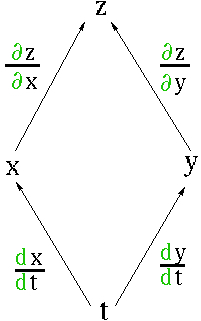
\includegraphics[width=0.25\columnwidth]{chainrule}
\caption{Multi-variate chain rule}
\label{fig:gallery} 
\end{figure}

\subsection{Proof of multivariate chain rule}


\end{document}